% Minuta para relatórios finais para a unidade curricular
% de "Estagio ou Projecto" do curso de Licenciatura em Engenharia Informática
% do Instituto Politécnico de Beja
% Versão de 2013/04/18
% Autor: João Paulo Barros, joao.barros@ipbeja.pt

\documentclass{ipbeja-trabalhos-academicos}
% Para preencher 

\newcommand{\ESCOLA}{Escola Superior de Tecnologia e Gestão}

\newcommand{\TITULO}{Business Intelligence - Open Source Driven}
\newcommand{\SUBTITULO}{Opcionalmente, colocar aqui sub-título com máximo de vinte palavras}
\newcommand{\TITLE}{Business Intelligence - Open Source Driven}
\newcommand{\SUBTITLE}{Put here the subtitle in english}


\newcommand{\CANDIDATO}{Emanuel Alexandre Cavaco Teixeira}

 %se for um projecto comentar a linha seguinte. Caso contrario indicar orientador
 % na entidade de acolhimento do estágio
\newcommand{\ORIENTADORENTIDADE}{Eng. Nuno Miguel Lopes dos Santos, Deloitte}
\newcommand{\ORIENTADORIPBA}{Nome completo do docente orientador e respectivo título académico}
% se não existir segundo orientador do IPBeja, comentar a linha seguinte
\newcommand{\ORIENTADORIPBB}{Nome completo do segundo docente orientador respectivo título académico} 


%Completar e comentar um dos seguintes dois \newcommand
%\newcommand{\DECLARACAOPROJETO}{Relatório de projeto de fim de curso apresentado na\linebreak \ESCOLA{} do Instituto Politécnico de Beja}
\newcommand{\DECLARACAOESTAGIO}{
Relatório de estágio, realizado na Deloitte, apresentado na\linebreak \ESCOLA{} do Instituto Politécnico de Beja}

% commentar se não existente
\newcommand{\DEDICATORIA}{dedication text}


\begin{document}
\folhacapa % 2.1 das normas
\folharosto % 2.3 das normas
%%%%%%%%%%%%%%%%%%%%%%%%%%%%%%%%%%%%%%%%%%%%
\frontmatter % parte inicial

\chapter{Resumo}
\section*{\textit{\TITULO}\\  {\small{\textit{\SUBTITULO}}}}

\par Este documento serve para descrever o trabalho realizado no âmbito da unidade curricular de Estágio e Projecto da Licenciatura de Engenharia Informática do Instituto Politécnico de Beja. O trabalho realizado consistia na construção de dashboards e gráficos sobre informações de gestão sobre receitas de tráfego, afectas ao ramo de negocio da empresa xpto. Esta informação será disponibilizada sob a forma de widgets para posteriormente serem incluídos no portal corporativo já existente.
\par A implementação destas funcionalidades foi efectuada através de tecnologias totalmente open source, fazendo com que esta informação chegue a um numero considerável de utilizadores, sem aumentar os custos de licenciamento inerentes a sistemas de reporting actualmente em uso na empresa xpto. Paralelamente a informação dos dashboards foi complementada com a inclusão de novas métricas e indicadores recorrendo ao QlikView. Isto permite uma visualização mais detalhada da informação, contudo menos acessível, devido aos custos de licenciamento.
\par Para além das tarefas supracitadas foi também desenvolvido um relatório em formato de newsletter na aplicação de report QlikView, e todo o processo de desenvolvimento estará descrito no presente documento.\newline

\textbf{Palavras-chave}: \textit{JavaScript, D3.js, AngularJS, JAVA, QlikView}.
\chapter{Abstract}
\section*{\textit{\TITLE}\\  {\small{\textit{\SUBTITLE}}}}

\textit{Between 100 and 200 words.}

...

...



\textbf{Keywords}: \textit{Specify between 5 and 10 keywords, separated by commas, about the theme of the report}.

% Se pretender remover, comente a linha seguinte, caso contrário preencha o ficheiro agradecimentos.tex
\agradecimentos

texto de agradecimento




\indicegeral  
\indicedefiguras % só se existirem mais do que 5 figuras. Caso contrário, remova.
\indicedetabelas % só se existirem mais do que 5 tabelas. Caso contrário, remova.
\indicedelistagens % só se existirem mais do que 5 listagens

% No caso de se verificar "um número significativamente elevado de abreviaturas e siglas" deve retirar-se o 
% comentário da linha seguinte e preencher o ficheiro parte-inicial/abreviaturas.tex
%\chapter{Abreviaturas e Siglas}
\begin{quote} % para uma pequena indentação
\begin{tabular}[t]{p{4cm} p{10cm}}


IPBeja & Instituto Politécnico de Beja\\
UML & Unified Modelling Language\\
....... & .....



\end{tabular}

\end{quote}
 

%%%%%%%%%%%%%%%%%%%%%%%%%%%%%%%%%%%%%%%%%%%%
\mainmatter  \pagestyle{ruled} % parte principal

\chapter{Introdução}
\label{intro}

\section{Âmbito}

\par O estágio foi concretizado na empresa de auditoria e consultoria Deloitte, nas instalações da Brisa, cliente da Deloitte, inserido na unidade curricular de Estágio ou Projecto, integrante do plano de estudos do curso de Licenciatura em Engenharia Informática da ESTIG, estabelecimento de ensino pertencente ao IPBeja. O trabalho concretizado no estágio contém um nível de dificuldade e complexidade adequado ao mercado de trabalho atual e face as funções que se pretende que um recém-licenciado na área da engenharia informática realize numa empresa de consultadoria. Convém reforçar ainda que as tecnologias utilizadas na concretização do estágio podem atualmente ser consideradas como “state-of-the-art” dado que se tratam de tecnologias muito recentes. O estágio realizado obedeceu aos seguintes pressupostos que tinham sido previamente estabelecidas com os responsáveis do IpBeja e da instituição de acolhimento:
\vspace{-0mm}
\begin{itemize}  \itemsep1pt \parskip0pt \parsep0pt
 \item Duração e Carga Horária: o estágio de duração mínima de três meses, com uma carga horária que se assemelhasse ao verdadeiro mercado de trabalho, cerca de 8 horas diárias, totalizando um total de quarenta horas semanais;
 \item Orientação curricular: Ser orientado por uma figura de mérito reconhecido dentro da instituição, bem como um docente pertencente à ESTIG com o intuito de supervisionar o trabalho realizado na instituição de acolhimento. Na instituição de acolhimento pude contar com o Eng.º Nuno Santos, Senior Manager da área de Consulting da linha de serviço de Application Management Services. Convém salientar que o trabalho operacional diário foi ainda supervisionado por um recurso sénior da instituição, em concreto, pelo team leader Mário Pereira, de acolhimento e pelos responsáveis da Brisa.  A Professora Doutora Isabel Sofia foi a docente do IpBeja responsável por acompanhar o meu trabalho.
\item Aprovação Prévia: obtenção prévia da aprovação do conteúdo e planeamento do estágio a que me propunha, por parte da Comissão de Estágios da LEI. A aprovação foi obtida na data DD-MM-YYYY.
\end{itemize}

\section{Instituição de acolhimento}

\par “Deloitte” é a marca sob a qual dezenas de milhares de profissionais, trabalhando em firmas independentes espalhadas por todo o mundo, colaboram na prestação de serviços de auditoria, consultoria de negócios e de gestão, corporate finance e gestão do risco, consultoria fiscal e serviços relacionados a clientes nos mais diversos setores de atividade.
\par A Deloitte surgiu em 1845 em Londres, sendo hoje uma das maiores empresas no mundo no seus sectores de atividade.
\par A marca “Deloitte”, surge em 1845 em Londres, e atualmente está espalhada pelo mundo, estando presente em mais de 150 países, com cerca de 700 escritórios e mais de 210.000 (duzentos e dez mil) colaboradores. Sobre a marca “Deloitte” operam firmas independentes, cada firma presta serviços numa determinada área geográfica e está restrita à legislação dessa mesma área geográfica onde opera.
\par Em Portugal a entidade membro da Deloitte é a Deloitte \& Associados, SROC S.A. Desta entidade legal fazem parte três subsidiarias que operam em ramos de negócio distinto, sendo que este projecto foi realizado ao serviço da SGG, Serviços Gerais de Gestão, S.A., que se dedica a comercializar serviços de Outsourcing nas áreas de contabilidade administrativa e consultoria geral, incluindo serviços de application management services,  na mesma área.
\par Em Portugal a Deloitte \& Associados, SROC S.A. é responsável por empregar mais  2000 colaboradores, divididos por dois Escritórios, Lisboa e Porto. Detêm ainda dois escritório em Luanda (Angola) e presta serviços ainda em Cabo Verde, São Tomé e Príncipe e Moçambique. Saliento ainda que dada a presença mundial da Deloitte e normal os seus colaboradores participarem em projetos internacionais por todo o mundo.


\section{Estrutura do documento}

 % capitulo 1
\chapter{Enquadramento}
\label{cap2}

Este capítulo exemplifica a utilização de referências, figuras, tabelas e listagens.

\section{Projeto}
\par A Brisa solicitou a colaboração da Deloitte para o desenvolvimento de uma plataforma tecnologia que permita disponibilizar informação de gestão consolidada/agregada fazendo uso das suas base de dados de informação de gestão e fazendo uso exclusivo de tecnologias open-source. Desta forma, a Deloitte iniciou uma prestação de serviços com uma duração de 6 meses com a participação de uma equipa de dois recursos, com a minha participação durante três meses e com a supervisão de um gestor de projeto com vasta experiência em soluções de Business Intelligence. A equipa de projeto foi completada com a participação de dois gestores de projeto da Brisa. O planeamento do projeto foi definido fazendo uso de metodologias Agile por diferentes motivos, nomeadamente, a necessidade de concretizar ajuste rápidos ao nível tecnológicos e de arquitetura até a sua estabilização final e devido ao fato de estarmos a colaborar com o cliente na definição de indicadores e layout de dasboards e reports que permitam caraterizar o negócio da melhor forma.
\section{Objetivo}
\par No âmbito do estágio foi definido que a minha participação no projeto iria contemplar todas as fases e componentes do projeto, por forma, a ter uma perceção global e integrada de toda a plataforma. Esta abordagem permitiu ter a experiência de interagir diretamente com o cliente incluindo nas fases de definição de requisitos e de testes de aceitação. 
\par Como objectivo complementar ao projeto, mas não menos importante fui inserido numa equipa de desenvolvimento, com metodologias adequadas mercado de trabalho, contribuindo isto para o aumento das importantes soft-skils.
\section{Planeamento}
\par O projeto foi desenvolvido, como já referido, recorrendo a metodologias Agile. Foi distribuído por quatro fases de desenvolvimento distintas, com uma sequência de trabalhos associada a cada fase. Face ao planeamento inicial ocorreram alguns ajustes no decorrer do estágio para fazer face aos ajustamentos que o projeto careceu durante a sua fase de desenvolvimento, como podemos observar na Figura  \ref{fig:planeamentoFig}. 
\begin{figure}[!htb]
\centering
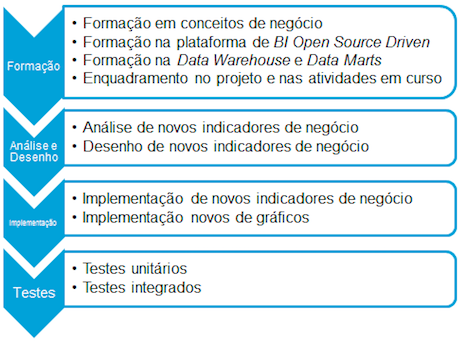
\includegraphics[width=9cm]{planeamento}
\caption{Planeamento}
\label{fig:planeamentoFig}
\end{figure}
\chapter{Título do Capítulo 3}
\label{cap3}

%a linha seguinte deve ser substituída pelo texto do capítulo
\lipsum

Mais umas citações \cite{AndroidTools, Chen1976}

% para adicionar o  capítulo N adicione a linha \input{capituloN} e crie o ficheiro 
% capituloN.tex na directoria "capitulos" 

% Bibliografia
%http://www.ieee.org/publications_standards/publications/authors/author_templates.html
\bibliographystyle{bibstyle-ipbeja}  
\bibliography{bibliografiaDoRelatorio}

%%%%%%%%%%%%%%%%%%%%%%%%%%%%%%%%%%%%%%%%%%%%%%%%
\apendices
\chapter{Título do Apêndice I}
\label{ap1}

%a linha seguinte deve ser substituída pelo texto do apêndice
\lipsum
% para adicionar o  apêndice N adicione a linha \input{apendiceN} e crie o ficheiro 
% apendiceN.tex na directoria "apendices" 

\anexos
\chapter{Título do Anexo I}
\label{an1}

%a linha seguinte deve ser substituída pelo texto do anexo
\lipsum
% para adicionar o  anexo N adicione a linha \input{anexoN} e crie o ficheiro 
% anexoN.tex na directoria "anexos" 

\end{document}